\subsection{Private Company Valuation}

\begin{figure}[H]
\centering
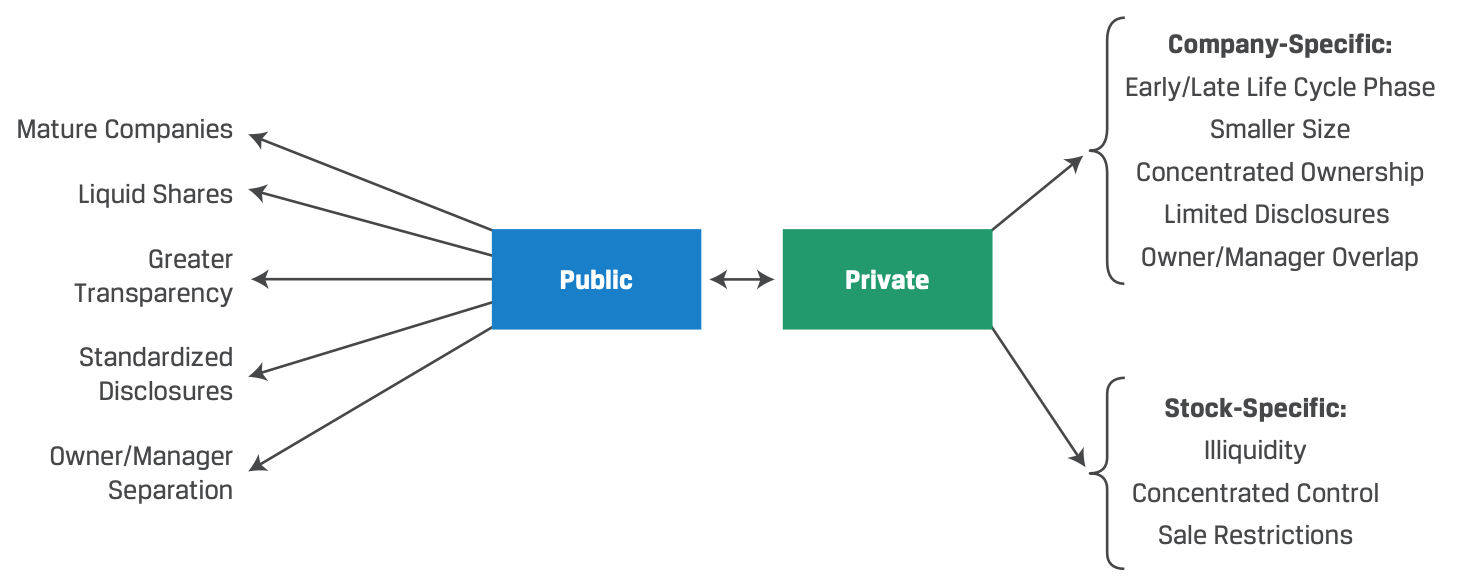
\includegraphics[scale=0.6]{/equity/pubvspriv}
\caption{Public vs Private Company Features}
\end{figure}

\begin{remark} \hlt{Company-Specific Features}
\begin{enumerate}[label=\roman*.]
\setlength{\itemsep}{0pt}
\item Stage of Life Cycle: private companies are typically less mature than public firms. In some circumstances, private companies are mature firms or bankrupt firms near liquidation. Valuation analysis vary with life cycle stage of the firm.
\item Size: Private firms typically. have less capital, fewer assets, fewer employees, hence are riskier. Thus private companies are valued using greater risk premiums and greater required returns. Lack of access to public equity markets may constrain private firm's growth, but regulatory burden associated with issuing public equity may outweigh benefit of greater access to funds.
\item Quality and Depth of Management: smaller private firms may not be able to attract as many qualified applicants as public firms, hence reducing the dept of management, slow growth and increasing risk.
\item Manager/Owner Overlap: in most private firms, management has substantial ownership position, reducing principal-agent conflict. External shareholders have little influence, allowing for longer-term perspectives.
\item Short-Term Investors: management in public firms take shorter-term view as compared to private firms where managers are long-term holders of significant equity interests.
\item Quality of Financial and Other Information: investor or creditor in a private firm will have less information than available for a public firm, leading to greater uncertainty, higher risk, reducing private firm valuation. Fairness opinions for private firm valuations relies on firm's financial statements and business records.
\item Taxes: private firms may be more concerned with taxes than public firms.
\end{enumerate}
\end{remark}

\begin{remark} \hlt{Stock-Specific Features}
\begin{enumerate}[label=\roman*.]
\setlength{\itemsep}{0pt}
\item Liquidity: private company equity has fewer potential owners and is less liquid than publicly traded equity. Hence a liquidity discount is often applied to valuing privately held shares.
\item Restrictions on Marketability: private companies have agreements to prevent shareholders from selling.
\item Concentration of Control: control of private firms is usually concentrated in hands of few shareholders, may lead to greater perks and other benefits to owners/managers at expense of minority shareholders.
\end{enumerate}
\end{remark}